\documentclass[10pt]{beamer} %
\usetheme{CambridgeUS}
% \usecolortheme{seahorse}
\usecolortheme{orchid}
% \usepackage[latin1]{inputenc}
\usefonttheme{professionalfonts}
\usepackage{times}
%\usepackage{tikz}
\usepackage{tikz}
\usetikzlibrary{chains}
\usepackage{pgfplots}
\pgfplotsset{compat=1.18} % Ensures compatibility for the plot
\usepackage{amsmath}
\usepackage{verbatim}
\usepackage{graphicx}
\usepackage{multicol}
%\usetikzlibrary{arrows,shapes}
\setlength{\tabcolsep}{20pt}
\renewcommand{\arraystretch}{1.5}

\usepackage{amsmath,amssymb,amsfonts}
\usepackage{hyperref}
\usepackage{textcomp}
\usepackage[english]{babel}
\usepackage{times}
% \usepackage[T1]{fontenc}

\usepackage{xcolor}
\usepackage{color, colortbl}
\usepackage{multirow}

%\usepackage{beamerthemesplit}
%\usetheme{Warsaw}
\setbeamertemplate{footline}[frame number]
%\usefonttheme{structurebold}
%\usefonttheme[onlymath]{serif}
%\usefonttheme{serif}
\usepackage{pgf}
\usepackage{amsmath,amssymb}
% \usepackage{inputenc}
%\usepackage[latin1]{inputenc}
\usepackage[english]{babel}
\usepackage{times}
\usepackage{hyperref}
\usepackage{colortbl}
\usepackage{helvet}
\usepackage{booktabs}
\usepackage{multirow}

\usepackage{tikz}
\usetikzlibrary{arrows,shapes,trees, positioning}
\usepackage{graphics}
\usepackage{color}

\pgfdeclarelayer{background}
\pgfdeclarelayer{foreground}
\pgfsetlayers{background,main,foreground}


%\usepackage[dvipsnames]{xcolor}
%\graphicspath{{images/}}
%\renewcommand{\baselinestretch}{1.5}
% \usepackage[utf8]{inputenc} % allow utf-8 input
% \usepackage[T1]{fontenc}    % use 8-bit T1 fonts
%\usepackage{listings}
%\usepackage{hyperref}       % hyperlinks
%\usepackage{url}            % simple URL typesetting
%\usepackage{booktabs}       % professional-quality tables
%\usepackage{amsfonts}       % blackboard math symbols
%\usepackage{nicefrac}       % compact symbols for 1/2, etc.
%\usepackage{microtype}      % microtypography
%\usepackage{lipsum}
% \usepackage{fancyhdr}       % header
%\usepackage{graphicx}       % graphics
%\usepackage{caption}
%\usepackage{subcaption}
%\usepackage[dvipsnames]{xcolor}
%\usepackage{cite}
%\usepackage{epsfig}
%\usepackage{textcomp}
%\usepackage{bm}
%
%\usepackage{algorithm}
%\usepackage{algorithmic}
%\usepackage{dsfont}
%\usepackage{appendixnumberbeamer}
%Header
% \pagestyle{fancy}
% \thispagestyle{empty}
% \rhead{ \textit{ }} 
% \setlength{\tabcolsep}{15pt}


\newcommand{\defn}{\textcolor{red}{Def:~}}
%\AtBeginEnvironment{frame}{\setcounter{myc}{0}}
\newcounter{myc}[section]%framenumber]
\newcommand{\expl}{\textcolor{blue}{\stepcounter{myc}Example~\arabic{myc}:~}}
\newcommand{\theo}{\textcolor{brown}{Theorem:~}}
\newcommand{\coro}{\textcolor{brown}{Corollary:~}}
\newcommand{\remark}{\textcolor{brown}{Remark:~}}
\newcommand{\sam}{\mathcal{S}}
\newcommand{\sig}{\mathcal{F}}
\newcommand{\R}{\mathbb{R}}
\newcommand{\bg}{\boldsymbol{g}}
\newcommand{\bX}{\boldsymbol{X}}
\newcommand{\bx}{\boldsymbol{x}}
\newcommand{\bY}{\boldsymbol{Y}}
\newcommand{\by}{\boldsymbol{y}}
\newcommand{\bt}{\boldsymbol{t}}
\newcommand{\bu}{\boldsymbol{u}}
\newcommand{\bmu}{\boldsymbol{\mu}}
\newcommand{\mc}{\{X_n:n\geq0\}}


\title[]{Statistical Inference and Multivariate Analysis (MA324)}
\subtitle{\textsc{Lecture Slides}\\Topic 05\\ Generalized Linear Regression}
\date{Jan-May 2026}


\graphicspath{{plots/}}

\AtBeginSection[]{
  \begin{frame}
  \vfill
  \centering
  \begin{beamercolorbox}[sep=8pt,center,shadow=true,rounded=true]{title}
    \usebeamerfont{title}\insertsectionhead\par%
  \end{beamercolorbox}
  \vfill
  \end{frame}
}

\begin{document}

% ===================================================================== Frame : Title Page
\thispagestyle{empty}
\maketitle

\section{Generalized Linear Regression}

\begin{frame}
    \frametitle{Introduction to GLMs}
    Ordinary Least Squares (OLS) regression assumes continuous, normally distributed outcomes. \textbf{Generalized Linear Models (GLMs)} extend this framework to accommodate non-normal distributions (e.g., binary, counts).
    
    \vspace{0.5cm}
    A GLM consists of three core components:
    \begin{enumerate}
        \item \textbf{Random Component:} The probability distribution of the response variable $Y$ (must belong to the exponential family).
        \item \textbf{Systematic Component:} The linear predictor $\eta = X\beta$.
        \item \textbf{Link Function:} A function $g(\cdot)$ that relates the expected value of $Y$, $\mu = E(Y)$, to the linear predictor: $g(\mu) = \eta$.
    \end{enumerate}
\end{frame}

\section{Logistic Regression}
\begin{frame}
    \frametitle{When to Use Logistic Regression}
    Logistic regression is used when the response variable $Y$ is \textbf{binary} or dichotomous (e.g., 0/1, Success/Failure, Dead/Alive).
    
    \vspace{0.5cm}
    \textbf{Why OLS fails for binary data:}
    \begin{itemize}
        \item \textbf{Non-normality:} The error terms cannot be normally distributed; they only take two possible values.
        \item \textbf{Heteroskedasticity:} The variance of a binomial distribution is $p(1-p)$, which changes as the probability $p$ changes.
        \item \textbf{Out-of-bounds Predictions:} OLS can predict probabilities $< 0$ or $> 1$.
    \end{itemize}
\end{frame}

\begin{frame}
    \frametitle{Logistic Regression: Theory}
    \begin{itemize}
        \item \textbf{Random Component:} $Y \sim \text{Bernoulli}(p)$, where $p = P(Y=1)$.
        \item \textbf{Link Function:} The \textbf{logit} function (log-odds).
    \end{itemize}
    
    \begin{equation*}
        \text{logit}(p) = \ln\left(\frac{p}{1-p}\right) = \beta_0 + \beta_1 X_1 + \dots + \beta_k X_k
    \end{equation*}
    
    \vspace{0.3cm}
    To solve for the predicted probability $p$, we use the inverse logit (logistic) function:
    
    \begin{equation*}
        p = \frac{\exp(X\beta)}{1 + \exp(X\beta)}
    \end{equation*}
\end{frame}

\begin{frame}
    \frametitle{MLE for Logistic Regression}
    Instead of OLS, logistic regression parameters are estimated using \textbf{Maximum Likelihood Estimation (MLE)}. 
    
    \vspace{0.3cm}
    For $n$ independent observations where $Y_i \sim \text{Bernoulli}(p_i)$, the probability function is $p_i^{y_i}(1-p_i)^{1-y_i}$. The \textbf{log-likelihood function} ($\ell$) is:
    
    \begin{equation*}
        \ell(\beta) = \sum_{i=1}^{n} \left[ y_i \ln(p_i) + (1 - y_i) \ln(1 - p_i) \right]
    \end{equation*}
    
    \vspace{0.2cm}
    We substitute $p_i$ with our model $\frac{\exp(X_i\beta)}{1 + \exp(X_i\beta)}$:
    \begin{equation*}
        \ell(\beta) = \sum_{i=1}^{n} \left[ y_i (X_i\beta) - \ln(1 + \exp(X_i\beta)) \right]
    \end{equation*}
    
    \textit{Note: There is no closed-form algebraic solution for $\beta$. Algorithms like Iteratively Reweighted Least Squares (IRLS) are used to find the maximum numerically.}
\end{frame}

\begin{frame}
    \frametitle{Interpreting Coefficients}
    Unlike OLS, coefficients in logistic regression represent changes in the \textbf{log-odds} of the outcome.
    
    \vspace{0.5cm}
    \begin{itemize}
        \item $\beta_1$: A one-unit increase in $X_1$ is associated with a $\beta_1$ increase in the \textit{log-odds} of $Y=1$.
        \item $e^{\beta_1}$ (\textbf{Odds Ratio}): A one-unit increase in $X_1$ multiplies the odds of $Y=1$ by a factor of $e^{\beta_1}$.
        \begin{itemize}
            \item If $e^{\beta_1} > 1$: The predictor increases the probability of the outcome.
            \item If $e^{\beta_1} < 1$: The predictor decreases the probability of the outcome.
        \end{itemize}
    \end{itemize}
\end{frame}

\begin{frame}[fragile]
    \frametitle{Applied Example: Logistic Regression}
    Using R's built-in \texttt{mtcars} dataset, let's predict if a car has a V-shaped engine (\texttt{vs} = 0) or a straight engine (\texttt{vs} = 1) based on its fuel efficiency (\texttt{mpg}).
    
\begin{verbatim}
# Fit the logistic regression model
logit_model <- glm(vs ~ mpg, data = mtcars, 
                   family = binomial(link = "logit"))

# View coefficients
coef(logit_model)
(Intercept)         mpg 
 -8.8330546   0.4304135 
\end{verbatim}
\end{frame}

\begin{frame}[fragile]
    \frametitle{Interpreting the Output}
\begin{verbatim}
# Extract the coefficient for mpg and 
# calculate the Odds Ratio
exp(coef(logit_model)["mpg"])
     mpg 
1.537898 
\end{verbatim}

    \vspace{0.5cm}
    \textbf{Interpretation:}\\ 
    For every 1 mpg increase in fuel efficiency, the log-odds of a car having a straight engine increase by 0.43.
    
    \vspace{0.3cm}
    Exponentiating this coefficient gives us an \textbf{Odds Ratio of 1.53}. This means that for every 1 unit increase in mpg, the odds of the car having a straight engine increase by 53\%.
\end{frame}

%%%%%%%%%%%%%%%%%%%%%%%%%%%%%%%%%%%%%%

\section{Poisson Regression}

\begin{frame}
    \frametitle{When to Use Poisson Regression}
    Poisson regression is used when the response variable $Y$ represents
    \textbf{count data} (e.g., number of hospital visits, number of traffic
    accidents).
    
    \vspace{0.5cm}
    Characteristics of count data:
    \begin{itemize}
       \item Discrete, non-negative integers $\left\{ 0, 1, 2, \dots \right\}$.
        \item Often right-skewed (many low counts, few high counts).
    \end{itemize}
\end{frame}

\begin{frame}
   \frametitle{Poisson Regression: Theory}
   \begin{itemize}
      \item \textbf{Random Component:} $Y \sim \text{Poisson}(\lambda)$, where $\lambda$ is the expected count (rate).
      \item The \textbf{PMF} is
         \begin{align*}
            P \left( Y=k \right) = \frac{e^{-\lambda} \lambda^k}{k!} \quad
            \text{for } k=0,1,2,\ldots.
         \end{align*}
      \item $E(Y) = \text{Var}(Y) = \lambda$.
   \end{itemize}
   \begin{center}
      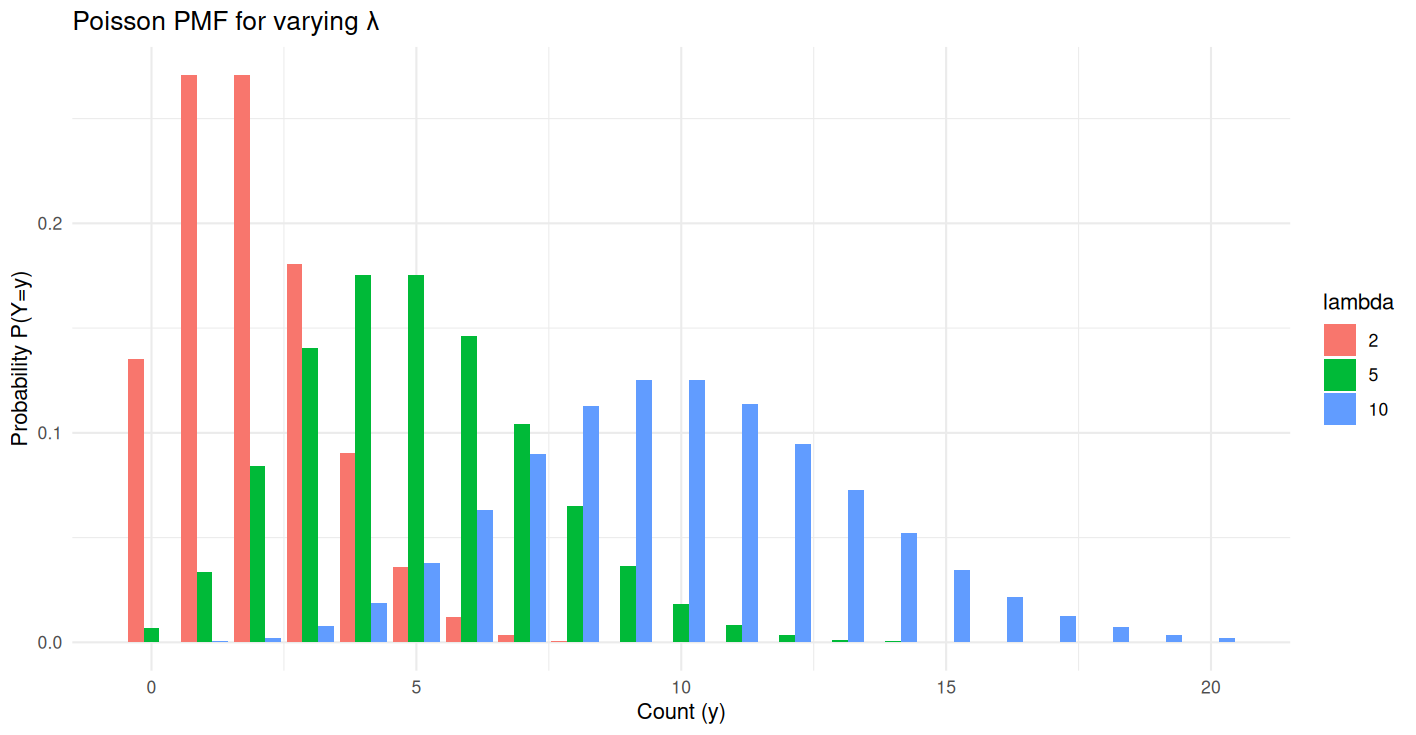
\includegraphics[width=0.8\textwidth]{poisson-plot.png}
   \end{center}
\end{frame}

\begin{frame}
    \frametitle{Poisson Regression: Theory}
    \begin{itemize}
       \item \textbf{Link Function:} The \textbf{natural log} function.
          \begin{equation*}
             \ln(\lambda) = \beta_0 + \beta_1 X_1 + \dots + \beta_k X_k = X\beta
          \end{equation*}
       \item To solve for the expected count $\lambda$, we exponentiate the linear predictor:
          \begin{equation*}
             \lambda = \exp(X\beta)
          \end{equation*}
    \end{itemize}
   \begin{center}
      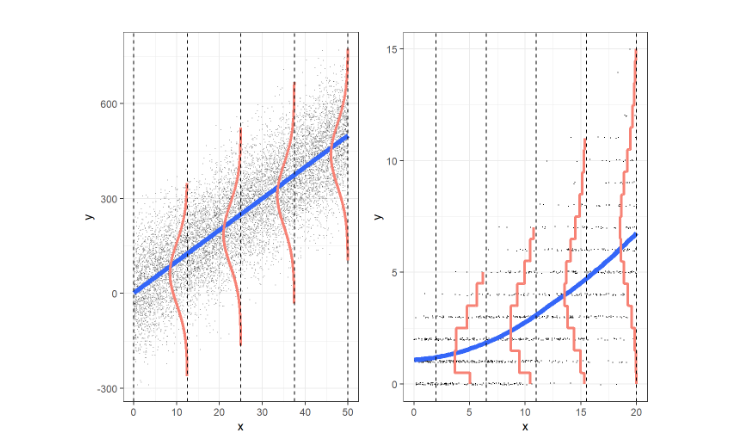
\includegraphics[width=0.8\textwidth, height=0.5\textheight]{LRvsPR.png}\\
      Comparison between LR and PR
   \end{center}
   \begin{flushright}
      {\tiny Source: https://bookdown.org/roback/bookdown-BeyondMLR/ch-poissonreg.html}
   \end{flushright}
 \end{frame}

\begin{frame}
    \frametitle{MLE for Poisson Regression}
    The \textbf{log-likelihood function}:
    
    \begin{equation*}
        \ell(\beta) = \sum_{i=1}^{n} \left[ y_i \ln(\lambda_i) - \lambda_i - \ln(y_i!) \right]
    \end{equation*}
    
    \vspace{0.2cm}
    We substitute the expected count $\lambda_i$ with our model $\exp(X_i\beta)$:
    \begin{equation*}
        \ell(\beta) = \sum_{i=1}^{n} \left[ y_i (X_i\beta) - \exp(X_i\beta) - \ln(y_i!) \right]
    \end{equation*}
    
    \textit{Note: As with the logistic model, we must take the derivative with respect to $\beta$ and use numerical methods (like IRLS) to solve for the maximum.}
\end{frame}

\begin{frame}
    \frametitle{Interpreting Coefficients}
    Coefficients in Poisson regression represent changes in the \textbf{log-count}.
    
    \vspace{0.5cm}
    \begin{itemize}
        \item $\beta_1$: A one-unit increase in $X_1$ is associated with a $\beta_1$ increase in the \textit{log-expected count}.
        \item $e^{\beta_1}$ (\textbf{Incidence Rate Ratio / IRR}): A one-unit increase in $X_1$ multiplies the expected count by a factor of $e^{\beta_1}$.
    \end{itemize}
\end{frame}

\begin{frame}
    \frametitle{Data Overview: The \texttt{warpbreaks} Dataset}
    To demonstrate Poisson regression, we will use R's built-in
    \texttt{warpbreaks} dataset. It records the number of warp breaks in yarn
    during weaving under different experimental conditions.
    
    \vspace{0.5cm}
    \textbf{Variables in the dataset:}
    \begin{itemize}
        \item \texttt{breaks}: (Numeric) The number of breaks per loom. This is
           our non-negative count response variable ($Y$).
        \item \texttt{wool}: (Factor) The type of wool used (Levels: A, B).
        \item \texttt{tension}: (Factor) The level of tension applied to the
           yarn (Levels: L, M, H for Low, Medium, High).
    \end{itemize}
    
    \vspace{0.5cm}
    \textbf{Modeling Goal:} \\
    To estimate how changing the \texttt{tension} level affects the expected count of yarn \texttt{breaks}.
\end{frame}

\begin{frame}[fragile]
    \frametitle{Applied Example: Poisson Regression}
    Using the \texttt{warpbreaks} dataset, let's model the number of warp breaks per loom (\texttt{breaks}) based on the level of \texttt{tension} (Low, Medium, High).
    
\begin{verbatim}
# Fit the Poisson regression model
poisson_model <- glm(breaks ~ tension, data = warpbreaks, 
                     family = poisson(link = "log"))

# View coefficients
coef(poisson_model)
(Intercept)    tensionM    tensionH 
  3.5945693  -0.3662283  -0.3175402 
\end{verbatim}
\end{frame}

\begin{frame}[fragile]
    \frametitle{Interpreting the Output}
\begin{verbatim}
# Calculate the Incidence Rate Ratios (IRRs)
exp(coef(poisson_model))
(Intercept)    tensionM    tensionH 
 36.3999996   0.6933446   0.7279361 
\end{verbatim}

    \vspace{0.5cm}
    \textbf{Interpretation:}\\
    The baseline category for tension is "Low". \\
    \vspace{0.2cm}
    The IRR for \texttt{tensionM} (Medium) is 0.69. This means that, compared to low tension, changing to medium tension multiplies the expected number of breaks by 0.69 (a 31\% decrease in breaks).
\end{frame}

\begin{frame}
    \frametitle{Some Extensions}
    In real-world data, the strict assumptions of these GLMs often fail. Advanced modeling techniques address these violations:
    
    \vspace{0.3cm}
    \begin{itemize}
        \item \textbf{Overdispersion:} If $\text{Var}(Y) > E(Y)$, the Poisson
           assumption is violated, leading to underestimated standard errors. \\
           \textbf{Solution:} Use Negative Binomial Regression or Quasi-Poisson
           models.
        % \item \textbf{Rates vs. Counts:} If the time or space over which
           % events are observed varies, model a rate. \textbf{Solution:} Add an
           % Offset term ($\ln(\text{Exposure})$).
        \item \textbf{Excess Zeros:} If data contains more zeros than the
           Poisson distribution allows. \\
           \textbf{Solution:} Zero-Inflated Poisson models.
    \end{itemize}
\end{frame}

%%%%%%%%%%%%%%%%%%%%%%%%%%%%

\section{References}

\begin{frame}
   \frametitle{References}
   \begin{itemize}
      \item https://bookdown.org/roback/bookdown-BeyondMLR/ch-poissonreg.html  
   \end{itemize}
\end{frame}

\end{document}
